\documentclass[tikz, border=8pt]{standalone}
\usepackage{xcolor}
\usetikzlibrary{arrows.meta, positioning, shapes.geometric, calc}
% ============================================================
% Shared style definitions for the DarwinsRNAHunt methods figures.
% \input this file from each diagram's preamble (after \usepackage{xcolor}
% and \usetikzlibrary{...}) so colours/styles stay consistent everywhere.
%
% Visual grammar used throughout:
%   - white box, single border   = external / raw resource
%   - white box, double border   = curated data artifact (output of a section)
%   - coloured box, single border = an internal processing step
%   - coloured/white, dashed border = Snakemake checkpoint (dynamic re-evaluation)
%   - white box, short-dashed border = static external file (not produced by the pipeline)
% ============================================================

% ---------- category colours (ColorBrewer Set3-style) ----------
\definecolor{catDefine}{HTML}{FFFFFF}
\definecolor{catSelect}{HTML}{FFFFFF}
\definecolor{catAcquire}{HTML}{FFFFFF}
\definecolor{catLocalize}{HTML}{FFFFFF}
\definecolor{catExtract}{HTML}{FFFFFF}
\definecolor{catCombine}{HTML}{FFFFFF}
\definecolor{catCluster}{HTML}{FFFFFF}
\definecolor{catModel}{HTML}{FFFFFF}
\definecolor{catValidate}{HTML}{FFFFFF}
\definecolor{catReport}{HTML}{FFFFFF}

% ---------- Kea Palette (defined for optional future restyling; unused for now) ----------
\definecolor{keaGreen}{HTML}{6C803A}
\definecolor{darkBrown}{HTML}{7B5C34}
\definecolor{lightBrown}{HTML}{AB7C47}
\definecolor{keaYellow}{HTML}{CCAE42}
\definecolor{keaOrange}{HTML}{D73202}
\definecolor{charcoal}{HTML}{272318}
\definecolor{lightGrey}{HTML}{D3CDBF}

\tikzset{
    font=\fontsize{7}{8}\selectfont,
    >={Latex[length=2mm,width=1.4mm]},
    every path/.style={thick},
    % internal processing step
    stage/.style={rectangle, rounded corners=2pt, draw=black, thin,
        minimum height=1.05cm, text width=3.6cm, align=center, inner sep=3pt},
    % external / raw resource (input)
    res/.style={rectangle, rounded corners=2pt, draw=black, thin, fill=white,
        minimum height=1cm, text width=4.2cm, align=center, inner sep=3pt},
    % static external file, not produced by this pipeline
    ext/.style={rectangle, rounded corners=2pt, draw=black!55, dash pattern=on 2.2pt off 1.6pt,
        thin, minimum height=0.85cm, text width=3.1cm, align=center, fill=white,
        font=\fontsize{6.3}{7.3}\selectfont, inner sep=2.5pt},
    % Snakemake checkpoint modifier (combine with stage/res)
    ckpt/.style={dashed, line width=0.9pt},
    % deliverable / output-artifact modifier: crosses a section boundary
    deliver/.style={double, double distance=1.2pt, line width=0.85pt},
    lbl/.style={font=\fontsize{8.5}{9.5}\bfseries\selectfont},
    sublbl/.style={font=\fontsize{7}{8}\itshape\selectfont},
    node distance=0.55cm and 2.6cm
}

\tikzset{edgelab/.style={font=\fontsize{6.5}{7.5}\selectfont\itshape, inner sep=1.5pt, align=center}}

\begin{document}
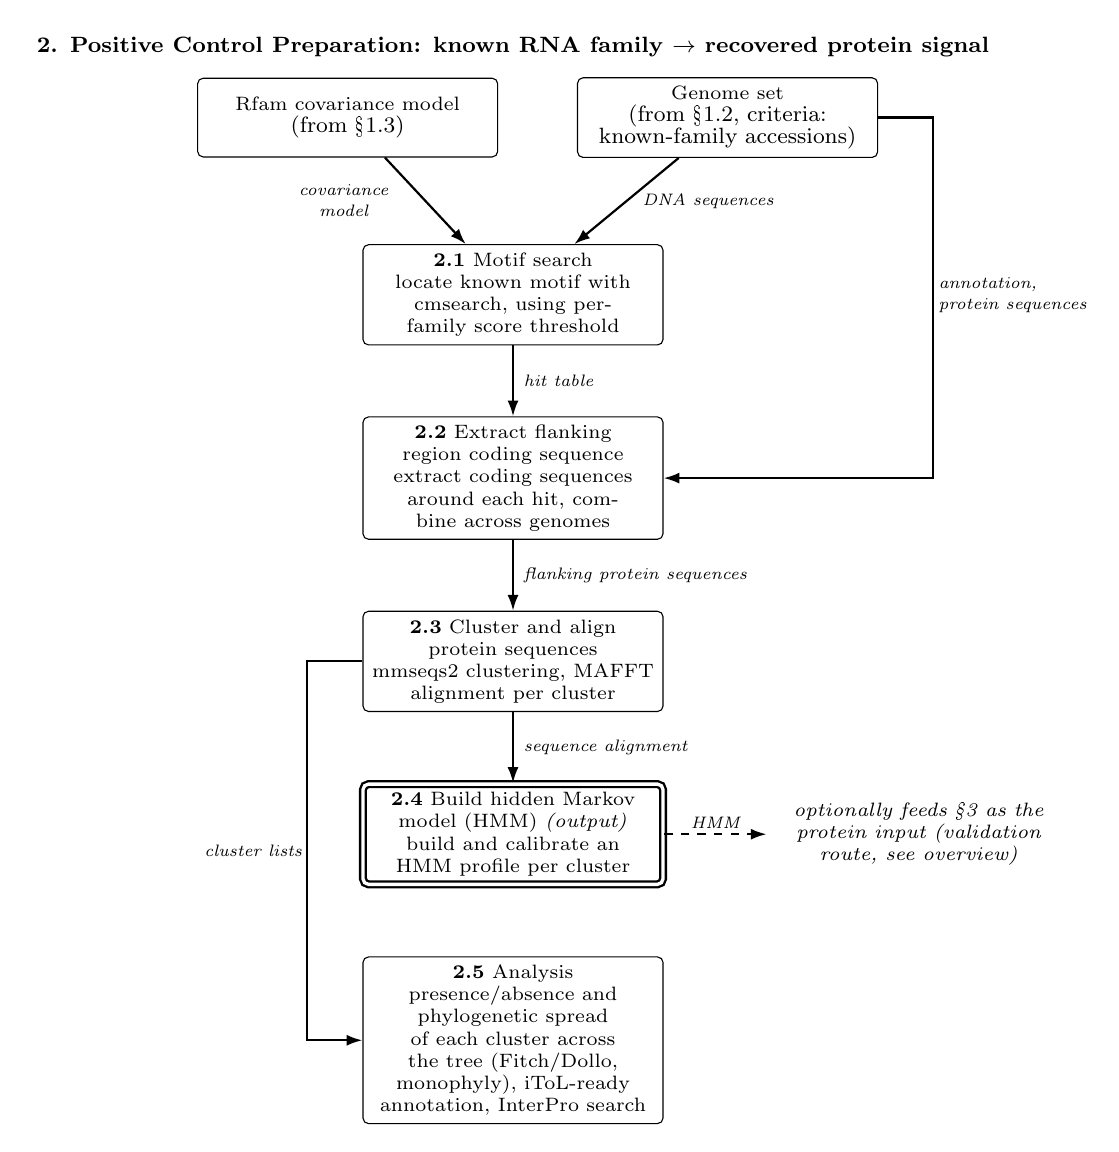
\begin{tikzpicture}

\node[lbl] (title) at (2.1,0.9) {2. Positive Control Preparation: known RNA family $\rightarrow$ recovered protein signal};

% ---------------- inputs (from \S1) ----------------
\node[res, text width=3.6cm] (in_rfam) at (0,0) {Rfam covariance model\\\footnotesize(from \S1.3)};
\node[res, text width=3.6cm, right=1.0cm of in_rfam] (in_genomes) {Genome set\\\footnotesize(from \S1.2, criteria: known-family accessions)};

% ---------------- pipeline chain ----------------
\node[stage, fill=catLocalize!70, below=1.1cm of in_rfam, xshift=2.1cm] (s21)
    {\textbf{2.1} Motif search\\locate known motif with cmsearch, using per-family score threshold};

\node[stage, fill=catExtract!85, below=0.9cm of s21] (s22)
    {\textbf{2.2} Extract flanking region coding sequence\\extract coding sequences around each hit, combine across genomes};

\node[stage, fill=catCluster!55, below=0.9cm of s22] (s23)
    {\textbf{2.3} Cluster and align protein sequences\\mmseqs2 clustering, MAFFT alignment per cluster};

\node[stage, deliver, fill=catModel!65, below=0.9cm of s23] (s24)
    {\textbf{2.4} Build hidden Markov model (HMM) \emph{(output)}\\build and calibrate an HMM profile per cluster};

\node[stage, fill=catValidate!55, below=0.9cm of s24] (s25)
    {\textbf{2.5} Analysis\\presence/absence and phylogenetic spread of each cluster across the tree (Fitch/Dollo, monophyly), iToL-ready annotation, InterPro search};

% ---------------- inputs -> 2.1 ----------------
\draw[->] (in_rfam) -- (s21) node[edgelab, midway, left=2pt, text width=1.8cm] {covariance model};
\draw[->] (in_genomes) -- (s21) node[edgelab, midway, right=2pt, text width=1.8cm] {DNA sequences};

% ---------------- genome set -> 2.2 (right-hand route) ----------------
\path let \p1=(s22.east), \p2=(in_genomes.east) in coordinate (rx) at ({max(\x1,\x2)+0.7cm},0);
\draw[->] (in_genomes.east) -- (rx |- in_genomes.east) -- (rx |- s22.east) -- (s22.east);
\node[edgelab, anchor=west, align=left] at (rx |- s21.east) {annotation,\\protein sequences};

% ---------------- chain ----------------
\draw[->] (s21) -- (s22) node[edgelab, midway, right=2pt] {hit table};
\draw[->] (s22) -- (s23) node[edgelab, midway, right=2pt] {flanking protein sequences};
\draw[->] (s23) -- (s24) node[edgelab, midway, right=2pt] {sequence alignment};

% ---------------- 2.3 -> 2.5 (left-hand route) ----------------
\coordinate (lx) at ($(s23.west)+(-0.7,0)$);
\coordinate (ly) at (lx |- s25.west);
\draw[->] (s23.west) -- (lx) -- (ly) -- (s25.west);
\node[edgelab, anchor=east, align=right] at ($(lx)!0.5!(ly)$) {cluster lists};

% ---------------- optional output to Section 3 ----------------
\node[sublbl, right=1.3cm of s24, text width=3.6cm, align=center] (opt)
    {optionally feeds \S3 as the protein input (validation route, see overview)};
\draw[->, dashed] (s24.east) -- (opt.west) node[edgelab, midway, above, text width=1.6cm] {HMM};

\end{tikzpicture}
\end{document}